\newpage
\section{Ejercicio 7}
	\subsection{Analisis del Schedler}

	Los quantums asignados a las colas de prioridad son 1 quatum a la de maxima prioridad y los argumentos pasados por parametro son las siguientes prioridades, de mayor a menor.

	Para entender el schedler, hemos corrido  una serie de tareas .

	\begin{figure}[ht]
		\begin{center}
			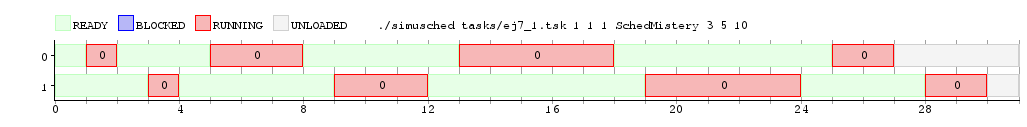
\includegraphics[width=1\columnwidth]{imagenes/ej7_1.png}
			\caption{Dos \texttt{TaskCPU} con 20 quantums.}
		\end{center}
	\end{figure}

	Se puede apreciar que cuando una  tarea acaba sus quantums, es quitada de la cola donde esta y es  agregada en la siguiente cola con menor prioridad , si es posible , en caso contrario quedara en la cola donde pertenece (La de menor prioridad) . Una vez que el schedler desencola todas las tareas pendientes en una cola pasa a la siguiente.


	\begin{figure}[ht]
		\begin{center}
			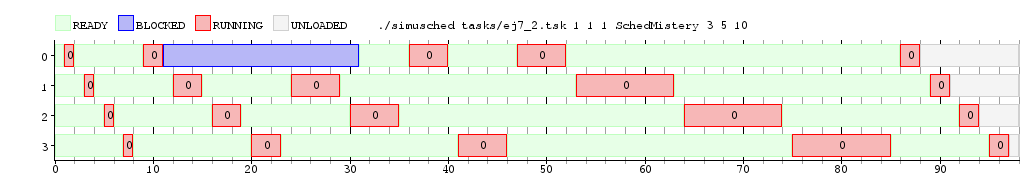
\includegraphics[width=1\columnwidth]{imagenes/ej7_2.png}
			\caption{Un \texttt{TaskCPU} corriendo con 20 quantums y tres \texttt{TaskAlterno} alterando 2 quantums de uso de kernel , 1 de bloqueo}
		\end{center}
	\end{figure}

	Como se puede apreciar este schedler permite starvation, Haciendo que las tareas con pocos ó ningun bloqueo se acumulen en las colas con menor prioridad, mientras dos ó más tareas de mayor prioridad, que se bloquen antes de que se les acabe el quamtum, se ejecuten y se pasen el control del kernel, entre ellas.
	Cuando una tarea se desbloquea , es la proxima tarea ha correr y su nivel de prioridad aumenta en uno.

	\begin{figure}[ht]
		\begin{center}
			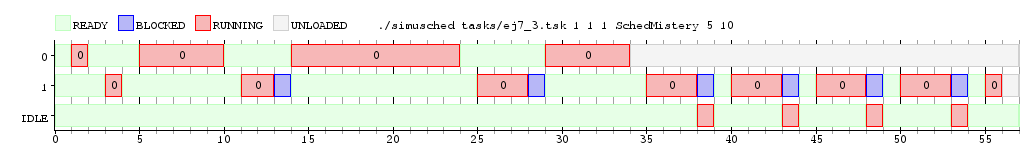
\includegraphics[width=1\columnwidth]{imagenes/ej7_3.png}
			\caption{Un \texttt{TaskCPU} corriendo con 20 quantums y un \texttt{TaskAlterno} alterando 2 quantums de uso de kernel , 1 de bloqueo al principio y despues 4 y 2.}
		\end{center}
	\end{figure}

	Como se ve la tarea IDEL  actua como se espera , cuando no hay nada para correr , corre la idle.

	

\newpage

	\subsection{Implementación del Schedler}

	\begin{itemize}
		\item \underline{Variables del Schedler}
			\begin{itemize}
				\item \textbf{vq} : Es un vector de colas de enteros, la cola de enteros para guardar los pid de las tareas a correr y el vector de colas, una para cada prioridad.
				\item \textbf{def\_quantum} : Es un vector de enteros, donde se albergaran las distintos quantums 	asignados a las distintas prioridades.
				\item \textbf{unblock\_to}: Es un vector de entero, donde cada proceso a travez de su pid guarda su nivel de prioridad en el momento de su último bloqueo.
				\item \textbf{n} : Es un entero que indica en que nivel de prioridad esta corriendo el schedler
				\item \textbf{quantum} : Es un entero que indica cuantos ticks le queda a la tarea actual, que 	esta corriendo el schedler
				\item \textbf{cur\_pri}: Es un entero que almacena el último pid que se acaba de desbloquear.
			\end{itemize}
		\item \underline{Funciones del Scedler}
			\begin{itemize}
				\item \textbf{SchedNoMistery} : Toma los argumentos pasados por parametro y se los 			asignados a def\_quantum. Instacia las demas varibles.
				\item \textbf{load}: Cuando una tarea entra en el schedler es agregada en la cola en la 	cual esta corriendó y es agregada en unblock\_to, por si en el futuro se bloquea.
				\item \textbf{tick} :Primero consulta si la tarea actual es la idle, ya que
					en ese caso se llama a next para saber quien sera la proxima tarea a correr
					. En caso de no ser la tarea idle, si el motivo del tick es un \texttt{TICK} se procede de una
					manera y si es \texttt{BLOCK} de otra y lo mismo con \texttt{EXIT}. 
					
					Si llega con motivo \texttt{TICK}, se decrementa en uno el quantum disponible, si le quedan quantums sigue la tarea actual, en caso contrario , la tarea que estaba corriendo es movida a la siguiente cola con menor prioridad, si se puede , en caso contrario quedara en la cola donde pertenece (La de menor prioridad).Luego se llama a \textbf{next}, para saber quien sigue y por ultimo se reinicia los quantums correspondientes a la cola actual del schedler.
					
					Si el motivo es \texttt{EXIT}, la tarea actual es desalojada
					dándole lugar a la próxima tarea llamando a \textbf{next} y reiniciando el quantum a su valor correspondiente a la cola actual del schedler.
					
					Si el motivo es \texttt{BLOCK}  , la tarea actual es desalojada 
					dándole lugar a la próxima llamando a \textbf{next}, luego se almacena el nivel de prioridad subido en uno en unblock\_to  y por último se  reinicia el quantum a su valor correspondiente a la cola actual del schedler.
				\item \textbf{next} : Devido a que saber quien es la proxima tarea a correr en el 			schedler es una necesidad repetida se paso a crear esta funcion.
					
					En caso que no haya ninguna tarea a correr , se devuelve la tarea idel.
					
					Si se desbloqueo una tarea se devuelve esa y el nivel de prioridad de schedler pasa a ser el guardado en unblock\_to con su pid; caso contrario se busca a travez de todas las colas , llendo de la prioridad actual a la menor , buscando la proxima tarea a ejecutar.

			\end{itemize}
	\end{itemize}




